\documentclass[12pt]{article}

\usepackage{fullpage}
\usepackage{graphicx, rotating, booktabs} 
\usepackage{times} 
\usepackage{natbib} 
\usepackage{indentfirst} 
\usepackage{setspace}
\usepackage{grffile} 
\usepackage{hyperref}
\usepackage{adjustbox}
\setcitestyle{aysep{}}


\singlespace
\title{\textbf{Alliance Treaty Design and the Arms-Alliances Tradeoff}}
\author{Joshua Alley\footnote{Graduate Student,
Department of Political Science, Texas A\&M University.}}
\date{{\normalsize \today}}

\bibliographystyle{apsr}

\begin{document}

\maketitle 

\newpage 

\doublespace 



\section*{Introduction}

How can states increase their security in international relations? States can augment their material capabilities and security through spending more on arms, or forming new alliances. Because states can use either arms or alliances to gain security, they can replace one policy with another. To reap economic and political dividends, states will often substitute alliances for arms, reducing their own defense effort as they gain the support of other states. 

Two strands of academic inquiry expect that alliance formation will lead to reduced arms spending. Theories of arms and alliances start with the premise that the two are substitute goods and increasing alliance ties will lead to decreasing reliance on arms \citep{Morrow1993, Sorokin1994, DigiuseppePoast2016}. Economic theories of alliances predict that small states will reduce defense effort and free-ride on the protection of more powerful partners in their alliance \citep{OlsonZeckhauser1966, SandlerHartley2001}. 

There is mixed statistical evidence for the prediction that alliances lead to reduced defense effort. Some studies find a negative association between alliances and arms spending \citep{Conybeare1992, Morrow1993, Kimball2010, DigiuseppePoast2016}, but others suggest that arms and alliances are positively correlated \citep{Diehl1994, Horowitzetal2017, MorganPalmer2006}. Positive correlations between arms spending and alliances are puzzling for theories that anticipate reduced defense expenditure after alliance formation.

The Triple Entente is a puzzling case for theories of substitution between arms and alliances. In the early 20th century, France, Russia and the UK formed an alliance network including three of the most capable states in the international system. But even after forming an alliance with France in 1904 and Russia in 1907, UK military spending rose from \textsterling 53207 thousand in 1907 to \textsterling 67957 thousand in 1912. Meanwhile, French military spending rose from \textsterling 38956 thousand  in 1904 to \textsterling 61367 thousand by 1912 \citep{SingerCINC1988}. For the members of the Triple Entente, new alliances did not lead to reduced defense effort \citep{Schmitt1924}. 

Another entente is a puzzling case for theories of arms and alliances. Between the World Wars, Yugoslavia, Czechoslovakia and Romania formed the Little Entente to balance Hungary and secure their new independence \citep{Benes1922, Osusky1934}. France formed alliances with all these states by 1921 to secure the new status quo in Eastern Europe \citep[pg. 142-3]{Crane1931}, but Czechoslovakian and Romanian military spending steadily increased from 1920 on before plateauing during the Great Depression and then increasing again until 1936, when the alliance broke down. France's substantial capability should have allowed the weaker members of the Little Entente to reduce their defense effort, but there is limited evidence they did. 

 

What determines the combination of arms and alliances states use to seek security? I argue that different institutional designs affect the credibility of alliance promises. Those differences in credibility affect the need for states to invest in domestic defense capacity to protect against abandonment. 
 
Whether international competition leads to alliances, military spending, or both has substantial ramifications for international and domestic prosperity and security. Military spending consumes resources that might otherwise be used for social welfare, creating a ``guns and butter trade off.'' According to the Stockholm International Peace Research Institute, less than 10\% of annual global military spending could fund the UN's Sustainable Development Goals for education \citep{SIPRI2016}. Alliances also generate security externalities beyond deterrence, including entrapment in war \citep{Snyder1984} and conflict diffusion \citep{MelinKoch2010}. 

This research encompasses several fields of inquiry in international relations. Alliances and military spending are often examined separately. Most empirical work on alliances uses a binary dependent variable--- states can either form an alliances or not. But if the alternative to an alliance is added military spending, rather than no alliance, our theories and empirical tests of alliance formation are incomplete. Determinants of military spending cannot be addressed in isolation from a state's alliance commitments \citep{Nordhausetal2012}.   

Understanding how states mix arms and alliances in their quest for security also contributes to scholarship on the political economy of armed conflict. War has shaped state coercive capacity \citep{Bean1973, Tilly1990}, tax policy \citep{Dinceccoetal2011, ScheveStasavage2012}, and central banking \citep{Poast2015}. Military spending and alliances determine the economic burden of providing security, making them integral concerns in the political economy of armed conflict.  

Trade offs between arms and alliances are relevant to the efficacy of different security policies. How states can mix arms and alliances will determine whether particular policy combinations can provide enough security at an acceptable economic burden. Clarifying the academic debate can therefore provide guidance about the future of international politics, including the viability of current alliance arrangements. 

US policymakers often complain that few of NATO's 28 members meet the defense spending obligation of at least 2\% of GDP. In 2011, US Secretary of Defense Robert Gates warned that NATO was becoming a ``two-tier alliance.'' If states consistently reduce arms spending after forming alliances, these warnings will have little effect. Most contemporary theories predict that states will use alliances to maintain their security while reducing spending on arms. 


\section*{Arms versus Alliances}

% Can summarize lit to date here. 

\citet{Altfield1984} and \citet{Morrow1993} noted that states can use arms or alliances to produce security, making them substitute goods. The economic theory of alliances predicts that smaller allies will ``free-ride'' on the security provided by their larger partners \citep{OlsonZeckhauser1966, SandlerHartley2001, Lake2009}. As a result, increasing alliance ties should lead to a reduction in arms spending. In accordance with these expectations, \citet{AllenDigiuseppe2013} find that states facing an sovereign debt crisis are more likely to form an alliances to maintain their security while reducing the economic burden of military spending. Substitution theory has a clear logic, but the empirical evidence is mixed. 

\citet{Diehl1994} finds that arms and alliances are positively associated, and \citet{Horowitzetal2017} show that states can use conscription to complement their efforts to form an alliance. However, states may only substitute arms for alliances with particular allies. \citet{DigiuseppePoast2016} argue that states are more likely to reduce military spending when they have a democratic ally, whose promises of support are more credible. 

States want to replace arms with alliances because of the guns and butter trade off in the domestic economy. Military spending consumes resources that could be used to provide other goods to society. \citet{Kimball2010} tests whether states with high levels of social demand use substitution and finds a positive correlation between infant mortality rates and alliance formation. This framework cannot explain why some states maintain high levels of both alliances and arms. What motivates states to carry a heavy economic and foreign policy burden through investment in both arms and allies? 

\section*{Theoretical Framework} 

I make three assumptions about the connection between alliance design and defense effort. The first assumption is that states are risk-averse over conflict, due to the consequences of losing a war. Following, \citet{Morrow1993}, I also assume that arms are a more reliable source of military capability, but that they are slower to develop than alliances. Alliances provide an immediate capability boost, but they are less reliable than domestic arms. Due to these differences, arms and alliances are imperfect substitute goods for states seeking security. 

In microeconomics, consumption of two goods depends on the marginal rate of substitution and the relative prices of those goods. The basic result in this framework is that individuals will consume as much as possible at the point where their indifference curves are tangential to the budget constraint. This point occurs when the marginal rate of substitution is equal to the ratio of the prices of these goods. The price ratio depends on the market price of each good, which in this case are the costs of arms and alliances. 

Most effort has been devoted to understanding the price of arms through the guns-butter trade off in the domestic economy. As arms become more costly, states are more likely to produce security through alliances. States with high costs of alliances will have more arms and less alliances. However, researchers have paid less attention to factors that alter the marginal rate of substitution, which reflects the extent to which alliances can substitute for arms. 

States can only reduce their defense effort if they believe that the promises of aid during war are credible. The regime type of allies is one possible source of alliance credibility \citep{DigiuseppePoast2016}. However, that is not the only possible source of credibility. 

Alliance treaties contain a wide range of terms, conditions, and obligations for signatories \citep{Benson2011, Chibaetal2015}. The content or institutional design of an alliance treaty determines its credibility. Put differently, the commitments states make through their alliances has consequences for the credibility of the treaty, and subsequent investment in arms by member states. Arms effort encompasses both military spending and personnel, though spending is the most common proxy. 

The scope of this theory is limited to the junior partners of major power states. These small states have strong incentives to reduce defense effort and ``free ride'' on the protection provided by larger states. By contrast, major powers have less incentive to free ride \citep{OlsonZeckhauser1966}, limiting their ability to trade off between arms and alliances. 


\subsection*{Alliance Design}
% A couple of paragraphs on alliance design considerations

Alliances provide for security cooperation, usually during or in anticipation of conflict. Once some conditions are met, the signatories are obligated to aid their treaty partners in conflict. Therefore treaty design informs both the probability of aid, and how much aid signatories can expect. Treaties that make high levels of aid more likely are therefore more valuable as a source of security. 

The conditions that trigger intervention by partners in an alliance vary widely across treaties and many are quite specific. Some pacts are open-ended, requiring engagement after any sort of hostilities commence. Other treaties stipulate narrow conditions for intervention, such as the set of belligerents and which state started the conflict. The scope or breadth of these conditions has important implications for understanding of whether a treaty has been honored \citep{Leedsetal2000}. 

Beyond the conditions for intervention, not all alliances stipulate a partner will become a belligerent in the conflict. For example, some alliances only promise consultation with the affected state. These limits on intervention help determine the value of the support to other partners, as participation in the fighting is usually more valuable than other support. 

In general, alliance treaties must balance between abandonment and entrapment \citep{Snyder1984, Benson2012}. General commitments to a robust intervention are highly credible, and reduce partner's fear of abandonment. However, general commitments also come with a risk of entrapment by creating a moral hazard for partners. 

Entrapment captures how alliance commitments can be used by states to drag their partners into conflicts they would rather avoid. Divergent foreign policy interests create a situation where one alliance partner sets the level of risk, but the other partners bear the costs. Greater foreign policy divergence makes states more likely to make limited alliance commitments, out of fear that their partners will entangle them in a war they have no interest in fighting \citep{Benson2012}. 

What are the implications of these differences between alliance treaties for domestic arms? Sufficient capabilities can deter an external threat, and arms and alliances are policy tools states use to augment their material capabilities. Domestic arms and external alliances are key sources of capability, but they are not perfect substitutes. 



\subsection*{Design and Credible commitments}
% Conditions and promised help determine costs of an alliance in expectation, and therefore its credibility

Domestic arms are a more certain means of offsetting a threat, so the expected contribution of arms to security is a state's total capabilities. Direct control of coercive resources makes domestic arms a highly credible source of capability for national leaders. By contrast, the capability gains from alliances are more uncertain, as they depend on the credibility of the treaty commitment. As the credibility of an alliance increases, the treaty becomes a better substitute for domestic arms. 

What makes an alliance commitment credible? Credible commitments have some costs associated with them, which allows observers to distinguish them from less meaningful ``cheap talk.'' Alliance treaties derive their credibility from the costs of violation and the expected costs of the promised intervention. 

Violating treaty commitments is costly due to lost reputation \citep{Gibler2008}, spill-overs to other commitments \citep{Crescenzi2012}, and audience costs \citep{Fearon1997, Tomz2007ar, Chibaetal2015, Levyetal2015}. Therefore, the greater the breadth of the commitments in an alliance, the more opportunities a state will have to violate those commitments, and the higher the potential cost. Broad commitments with few conditions attached to promises of military support also reflect high congruence in foreign policy interests. 

The other cost of an alliance treaty is the type of intervention it promises. An iron-clad promise to join a war is costly, due to the economic and political demands of war-fighting. Promises of consultation, or retaining the option to avoid fighting are less costly in expectation. Limited commitments allow an alliance partner to hedge its bets by withholding guarantees of full support. To the other members of an alliance, this commitment with less expected costs is not as reassuring. 

Alliance treaties that only promise support under a narrow set of circumstances, or do not guarantee active military support, are less credible. These alliances are less costly in expectation because they only cover a limited set of commitments, or they do not promise military engagement. As a result, partner states will view these security commitments more as ``cheap talk'' and adjust their defense policies accordingly. 

Less credible alliances increase the extent of imperfect substitution with arms. In expectation, states gain limited capability from less credible alliances, because they do not expect to receive the promised support. As a result, they must provide the capability to offset whatever threat they face by increasing or maintaining their defense effort.

All alliance members must hedge against the prospect of abandonment--- that their allies will not come to their aid in conflict. States that fear abandonment must plan for the worst and continue to maintain high levels of defense effort. Less credible alliance promises stoke fear of abandonment. Conversely, more credible promises of support increase the expected capability gains from an alliance, allowing states to shift domestic arms spending into other goods. 


\subsection*{Predictions}

My theoretical framework generates several testable predictions about the impact of alliance treaty provisions on members' defense spending. Substitution of arms for alliances is obvious when certain alliance characteristics are associated with reduced defense effort. Continuing to increase spending even after forming an alliance implies no substitution is taking place, as states keep their spending in line with economic growth/inflation or increase their defense effort. 

In general, complete alliance contracts that promise military support will lead to reduced defense effort. Not only are these alliances more credible, but they also cover many potential instances of conflict. Therefore, states can substitute and rely on the capability of their allies instead of maintaining high domestic defense effort to account for conflict risks that are not addressed by their alliances. Several scholars have classified alliances based on the conditions for support and the type of intervention. 

What types of alliances are most likely to reduce defense spending? And which alliance designs will be associated with no change in spending? \citet{Benson2011, Benson2012} divides alliances into unconditional, conditional, pure conditional and probabilistic commitments based on the content of the alliance agreement, which is a useful starting point. 

Probabilistic alliances do not guarantee military support even if the conditions for intervention are triggered. Either through delegation of the final intervention decision to another actor or escape clauses, probabilistic alliances augment uncertainty over whether the alliance partner will intervene. The lack of guaranteed military support is also a major concern for partners. Therefore, probabilistic alliances are unlikely to lead to substitution between alliances and arms, because they are less credible. Given uncertainty over whether they will actually receive support from their treaty partners, members of probabilistic alliances must maintain their defense effort to hedge against abandonment. 

\begin{quote}
\textsc{Hypothesis 1}: Probabilistic alliances will be associated with no change in defense spending by member states. 
\end{quote}

Unconditional alliances are more credible than probabilistic pacts. In an unconditional alliance, military support does not depend on specific conditions being met. Instead, the partners promise intervention irrespective of how the conflict arose. These alliances are highly credible due to their breadth and promises of military support. That credibility will lead member states to reduce their defense effort. 

\begin{quote}
\textsc{Hypothesis 2}: Unconditional alliances will be associated with decreases in defense spending by member states. 
\end{quote} 

It is more difficult to make clear predictions about conditional alliances. While these pacts promise military support, their credibility is reduced by the limited breadth of the conditions. The scope of the conditions that trigger intervention also varies widely across treaties. The most important concern for states seeking security from an external threat is whether their alliance covers the most important threats. Many conditional pacts may not address some threats, which reduces their value. The net impact of conditional alliances will often be close to zero, making conditional alliances a useful set of comparison cases for probabilistic and deterrent alliances. 

Alliance designs are highly strategic. The characteristics of partner states determine whether they form an alliance and how those treaties are designed. Because they face higher audience costs for reneging on their commitments, democracies are more likely to form alliances that only obligate them to consult with a partner, or specify limits to their defensive obligations \citep{Chibaetal2015}. Shared interest and the level of threat faced by a client state may explain why some clients get unconditional defense pacts \citep{Yarhi-Miloetal2016}. Accounting for the process of alliance formation helps address a potential objection to the theory.

An alternative to these predictions builds on the idea that weak commitments are designed to avoid generating entrapment and moral hazard \citep{Benson2012}. Ambiguous commitments restrain protege states from aggressive foreign policies by generating uncertainty about whether the patron will support them. But if a protege states is restrained by an uncertain treaty, might they then reduce military effort? States seeking conflict have every reason to increase defense spending, but if they can only rely on alliances for protection, they have more incentives to free ride. 

For this alternative explanation to hold, the increased risk of conflict from an uncertain commitment must be less than the decreased risk of conflict from reduced moral hazard. Otherwise, the overall risk of war will increase, and the members of an alliance will increase their defense effort. The strategic imperatives of alliance design make these changes unlikely. 

States that receive a highly uncertain commitment are likely to be in rivalry or some ongoing dispute that generates the moral hazard. Irrespective of the lost moral hazard from an ambiguous commitment, that rivalry is likely to continue. As a result, while they may lose the ability to provoke a favorable conflict, these states will still value deterrence from their alliances. However, the credibility of deterrent promises from their allies will be weakened, and these states will need to maintain higher levels of defense effort.

Another theoretical narrative that produces the opposite prediction of my framework emphasizes the role of regime type. If democracies are more likely to form alliances that only obligate them to consult with partners, or limit their commitments, but are generally reliable partners \citep{Chibaetal2015, DigiuseppePoast2016}, then limited commitments might lead to reduced defense effort. This alternative requires that the high credibility of those limited commitments is more important than the constrained support, and can be controlled for in an empirical analysis. Including democracy and alliance design considerations in the same model will likely provide a better picture of the effect each variable has on defense effort. 

There is an important scope condition to my theory. The dynamics I describe above apply primarily to smaller states, not to major powers. Many alliances are highly asymmetric, and the more capable partner is unlikely to reduce military spending after forming an unconditional deterrent alliance with a small state. Any association between alliance design and major power military spending would apply only to alliances between peers. Therefore, I focus my attention on non-major powers in the empirical test of the theory. 

Careful empirical design is necessary to accurately estimate the impact of alliance characteristics on defense spending. Attention to the structure of alliance data is perhaps the most important concern, and control variables can account for many of the strategic concerns around alliance designs In the next section, I describe my research design. 
 

\section*{Research Design} 

I test my two predictions on a sample of non-major powers in the international system from 1950-2001, which includes all states besides the Correlates of War project's list of major powers.\footnote{China, France, Russia, the UK, US as well as Japan and Germany after 1990 are the major powers I removed from the sample.} While this sample has limited temporal coverage, it means my results are comparable to work by \citet{DigiuseppePoast2016} and \citet{Nordhausetal2012}.\footnote{These other samples are limited by the availability and quality of economic indicators.} Using the same sample is especially helpful for comparison because I use a different estimator from most studies of the relationship between arms and alliances. 

Most studies of the arms-alliances tradeoff estimate regression models on state-year panel data. Researchers then use averages or dummy variables to summarize key characteristics of each state's total alliance portfolio. For example, \citet{Benson2012} uses a dummy variable to indicate if the state that initiated a militarized interstate dispute (MID) had a conditional alliance. \citet{DigiuseppePoast2016} use a dummy indicator of whether a state has at least one defensive alliance tie with a democratic state. Other studies aggregate the total capability of a state's allies \citep{Nordhausetal2012}. Both approaches limit our ability to make inferences about how differences in alliances affect state behavior. Dummy variables are particularly problematic because they can generate misleading comparisons between states by treating a state with at least one type of alliance as equivalent to states with many of the same type of treaties. 

Averaging or the use of dummy variables at the state-year level eliminates important variation between alliances. Without an explicit model of between alliance variation, there may be too much certainty in parameter estimates \citep{McElreath2016} because state level measures reduce the amount of variation in alliance-level variables. This is especially problematic for my theory, which emphasizes differences in \textit{alliance-level} characteristics. 

Therefore, I use a multiple membership multilevel regression model, which simultaneously models variation among observations clustered within alliances, states and years. Multilevel modeling allows me to directly model the impact of alliance-level covariates on state-level outcomes \citep{GelmanHill2007}. Multilevel models also account for sampling imbalance between groups by pooling strength and shrinking estimates towards an overall average. Applying a partial pooling approach also allows me to estimate the amount of variation in spending between alliances and states, and borrow strength for alliances with limited variation in membership over the sample. 

Hierarchical models are the most well-known type of multilevel model, where units are nested inside one another. State membership in alliances is less neatly organized--- many states are members of multiple alliance treaties, and different states are clustered within each treaty. Such multiple-membership data requires a slightly more complicated model. 

Using a multilevel model has some costs. Defining a separate regression for each level of the data requires additional assumptions about the distributions characterizing of state and alliance clusters \citep{McElreath2016}. Also, these models are computationally intensive and more difficult to estimate.

This model predicts annual military spending by non-major power states as a function of state and year varying intercepts, state-level variables, and the weighted sum of spending by other states in its alliances. Alliance characteristics predict the importance of spending by the other members of a particular treaty to each member. Therefore, I directly link a wide range of alliance treaty characteristics and military spending. 

\subsection*{Variables} 

The dependent variable is the log-transformed value of a state's military expenditures during each year. I also included a lag of the dependent variable, so that the model is equivalent to estimating changes in expenditure \cite{DeBoefKeele2008}. Using a lagged DV also allows direct estimates of the speed and extent of adjustments in spending. Expenditures change slowly over time, and I am estimating a partial adjustment model that implies changes in the independent variables will start an adjustment process that ends in a new equilibrium, ceteris paribus. Estimating changes directly imposes the assumption that unconditional alliances lead to negative changes as long as they are active, with no return to equilibrium. 

Military expenditure is the most common proxy for defense effort. Following \citet{DigiuseppePoast2016} I use data from \citet{Nordhausetal2012} who combine data from the Stockholm International Peace Institute (SIPRI) and Correlates of War (COW) projects to address defects in each.\footnote{SIPRI tends to under report spending by Warsaw Pact nations during the Cold War, while the COW data has some instances of measurement error.} The log transformation ensures the data are somewhat normally distributed for a regression estimator. 

I draw on two databases for measures key alliance characteristics. To test Hypotheses 1 and 2, I use the alliance classification of \citet{Benson2012}, who classifies alliances as probabilistic, conditional, or unconditional. In my sample, there are 38 unconditional, 30 probabilistic, and 80 conditional deterrent alliances. All 12 compellent alliances are unconditional and also have unconditional deterrent conditions. 179 alliances do not have any of Benson's conditions. All state alliance membership data and other important characteristics come from classifications come from the ATOP project \citep{Leedsetal2002}. 

Accounting for state and alliance characteristics that may be correlated with both alliance design and military expenditures is necessary to avoid omitted variable bias in the estimates. At the alliance level, I include binary indicators of whether an alliance stipulates military aid, is a bilateral treaty, and if any member was involved in a war. I also include the average democracy of the alliance members at the time of formation which is associated with alliance design \citep{Chibaetal2015} and spending by member states \citep{DigiuseppePoast2016}. Last, I control for superpower support with dummy indicators of whether the US and Russia were memebrs of the alliance.  

Controlling for some other types of alliances changes the interpretation of the key independent variables by altering the comparison category for each binary variable. While testing the impact of probabilistic and unconditional alliances, I control for whether an alliance has compellent aims and conditional deterrent alliances. Therefore, the remaining 179 alliances that make no specific promises of support are the base category. Following previous work, I remove non-aggression pacts from the alliance sample, so these alliances are mainly pacts that promise only consultation, or both consultation and non-aggression. 

The first set of state-level controls addresses the geopolitical environment for each state. Dummy indicators of participation in international war or civil war capture conflict participation, which can make defense a superior good \citep{OlsonZeckhauser1966}. I also include the military expenditures of rival states and a dummy variable indicator of Cold War years in the sample to measure potential arms competition. The natural log of GDP, and the POLITY measure of political institutions control for key domestic characteristics \citep{FordhamWalker2005}. GDP, POLITY, and rival military expenditures are all standardized for ease of interpretation. 


\subsection*{Model Details}

Varying intercept parameters encode the different clusters of observations in a multilevel model. These parameters are essential to modeling variance among groups within the data. Varying intercepts provide partial pooling among observations, which reduces the risk of maximally over or underfitting the data. I include an overall intercept parameter along with random intercepts for years, states, and alliances. The varying intercept parameters capture the deviation of each state, year, and alliance from the overall mean. The alliance-level intercepts are a function of the alliance-level variables. 

The dependent variable has a mean and median of 6.7, and half the observations fall between 5.2 and 8.2. The data itself has heavy tails, as some larger countries spend a great deal in a given year, and smaller states spend very little. The largest and smallest values are more than 3 standard deviations away from the mean, and there are more observations in the tails than a standard normal distribution. To ensure that the distribution of the outcome places adequate weight in the tails, I use a student's t distribution \citep{JuarezSteele2010}.\footnote{Fitting the model with a normally distributed outcome leads to poor performance for LOO and WAIC model comparison, which is further evidence that a a robust model is necessary \citep{Vehtarietal2017}}  The degrees of freedom parameter $\nu$ is estimated directly from the data using a diffuse gamma prior.

Formally, the full model can be expressed as follows, starting with state-year changes in the natural log of military spending $y_{it}$:
\begin{equation}
y_{it} \sim student_t(\nu, \mu, \sigma) 
\end{equation}

The mean of this distribution $\mu$ is a linear function of the overall mean $\alpha$, a state varying intercept $\alpha^{st}$, a year varying intercept $\alpha^{yr}$, a matrix of state-level regressors $W_{it}$ with a vector of parameters $\gamma$. The impact of alliance membership on military spending is the weighted sum of allied capabilities. The alliance-level variables predict the weight of each alliance. 

In the model, I connect alliance membership and military spending by multiplying a column vector of alliance weights by a row vector of state $i$'s alliance memberships at time $t$ $Z_{it}$. The columns of $Z$ correspond to individual alliances, marked by their ATOP id. Each element of $Z_{it}$ is equal to the total log-transformed military spending of all other states in an alliance if a state is a member of an alliance in a given year. All other elements of the membership matrix are zero. The non-zero values are rescaled by two standard deviations to facilitate model fitting.\footnote{Having parameters with different scales creates large differences in posterior variance, which makes posterior sampling more difficult.} Using alliance spending means that membership in different alliances is not treated equally. The full state-level model is:

\begin{equation}
\mu_{it} = \alpha + \alpha^{st} + \alpha^{yr} + W_{it} \gamma + Z_{it} \lambda 
\end{equation}

The varying intercepts capture state, year, and alliance-specific deviations from the overall mean. I assume that each alliance weight $\lambda_k$ is normally distributed, with mean $\theta_k$ and variance $\sigma^{all}$. $\theta_k$ is predicted by a second-level regression using the alliance characteristics. Therefore:

\begin{equation}
\lambda_k \sim N(\theta_k , \sigma^{all})
\end{equation} 
and 
\begin{equation}
\theta = X \beta
\end{equation}

The regressors in the alliance-level model predict the weight of that alliance's capability for state spending. Because my theory addresses the impact of alliance design on military spending, the $\beta$ parameters are the primary quantity of interest. The state-level variables control for state characteristics that also affect military spending. 

Consider one observation from Argentina as an example of how the model works. Argentine military spending in 1955 depends on Argentina's GDP, regime type, and other variables, as well as one intercept for Argentina and a year intercept. In 1955, Argentina was a member of two ATOP alliances- the Rio Pact and the Organization of American States (OAS). So Argentina's spending in 1955 also depended on the total spending of all other Rio Pact and OAS members. The importance Argentina places on that allied spending was a function of the design of the two treaties--- the Rio Pact is probabilistic deterrent, while the OAS is a conditional deterrent pact. 

\subsection*{Estimation and Priors} 

I estimate the model in \textsf{R} using STAN \citep{Carpenteretal2016}. STAN is a probabilistic programming language that supports full Bayesian inference, approximating the posterior distribution using Hamiltonian Monte Carlo (HMC). Fitting a multilevel regression model in the Bayesian framework requires clarity about the prior distributions. I have some information about the most likely coefficient values based on the scale of the data and the use of rescaled regressors, so weakly informative priors are appropriate \citep{Gelmanetal2014}. 

The range of plausible coefficient values can be captured without using heavy-tailed priors. Therefore, I use weakly informative normal priors with a mean of zero and standard deviation of one for the regression coefficients. Using heavier-tailed priors such as the Cauchy distribution on the coefficients in place of the normal priors is much more computationally expensive and can lead to nonsensical posterior predictions. Furthermore, the normal prior places 95\% of the prior weight on coefficient values between negative two and two, which does not rule out some large coefficients relative to the scale of the data. 

\autoref{tab:priors} summarizes all the prior distributions from the model. The estimated mean $\alpha$ is different from the mean of the data due to the inclusion of the lagged dependent variable. A normal prior with mean zero and standard deviation of three is diffuse enough to capture the overall mean and a wide range of other values besides that. 

I place half-normal priors with mean zero and a standard deviation of one on the variance hyperparameters in the model. Given the scale of the data, these priors are diffuse enough to allow for a wide range of pooling among states, years, and alliances. Larger estimates of the variance parameters imply that pooling assumptions for the different groups may be inappropriate. Fixed effects models, which assume no pooling, essentially impose an infinite estimate on the variance hyperparameters. 

The small scale on the gamma prior for the degrees of freedom parameter $\nu$ makes the prior diffuse enough to allow many possible distributions \citep{JuarezSteele2010}. As the degrees of freedom in a t-distribution decreases, more probability mass shifts out into the tails. A t-distribution with infinite degrees of freedom is equivalent to a normal distribution, on one hand, while the same distribution with one degree of freedom is equivalent to a Cauchy distribution. To avoid excessive posterior mass in the tails, and posterior predictions that far exceed the range of the observed data, I place a lower bound at four on the $\nu$ parameter. 


\begin{table} % Create a table of priors.

 \begin{center}
\begin{tabular}{c} 
$ p(\alpha) \sim N(0, 3)$  \\
$ p(\sigma) \sim \mbox{half-}N(0, 1) $ \\
$ p(\alpha^{yr}) \sim N(0, \sigma^{yr}) $ \\ 
$ p(\sigma^{yr}) \sim N(0, 1) $ \\
$ p(\alpha^{st}) \sim N(0, \sigma^{st}) $ \\ 
$ p(\sigma^{st}) \sim \mbox{half-}N(0, 1) $ \\ 
$ p(\sigma^{all}) \sim \mbox{half-}N(0, 1) $ \\
$ p(\beta) \sim N(0, 1) $ \\
$ p(\gamma) \sim N(0, 1) $ \\ 
$ p(\nu) \sim gamma(2, 0.1)$ 
\end{tabular} 
\end{center} 

\caption{Summary of Priors for Multilevel Model}
\label{tab:priors}
\end{table} 

A major limitation of the current model is that it does not account for time-varying alliance characteristics, such as changing democratic composition. Future work can address this issue. My theoretical focus on alliance design makes the focus on time-invariant characteristics acceptable for the moment- treaty conditions do not change over time without the alliance indicator changing in the ATOP data. 

There are 345 alliances in the sample, each with its own intercept parameter. In addition, all 49 years and 164 states have their own intercept. To facilitate estimation, I use a non-centered parameterization for the intercepts,\footnote{Also known as a standardized adaptive prior} which separates the hierarchical parameters out from lower-level model parameters \citep{McElreath2016}. The mean and variance of the intercept parameters are strongly correlated, which makes sampling from the posterior more difficult \citep{BetancourtGirolani2015}. Non-centered parameterization is another way of expressing the same model to improve sampling and protect the validity of inferences. 


\section*{Results} 

All the results reported below are based four chains which take 2,000 samples from the posterior distribution with a warm-up of 1,000 samples. All standard diagnostic tests indicate that the chains converged. There is adequate mixing in the chains, no divergent iterations, and the $\hat{R}$ statistic is well below 1.1 for all parameters.\footnote{See the appendix for more detail on these diagnostics.} I also validate the model fit using posterior predictive checking. 

There is some empirical support for my expectations. Unconditional pacts are associated with decreased military spending, while probabilistic deterrent and conditional deterrent pacts have no association with spending. \autoref{fig:post-prob} plots the posterior probability each coefficient is positive. 

\begin{figure}[htbp]
	\centering
  \includegraphics[width=0.95\textwidth]{C:/Users/jkalley14/Dropbox/Research/arms-allies/figures/post-prob.png}
	%\includegraphics[width=0.95\textwidth]{C:/Users/Josh/Dropbox/Research/arms-allies/figures/post-prob.png}
	\caption{Posterior Probability each model coefficients is positive. Precise posterior probability at the end of each bar.}
	\label{fig:post-prob}
\end{figure}


There is only a 6.6\% chance that conditional alliances are associated with increased spending. Probabilistic deterrent and conditional deterrent pacts have a 25\% and 28\% positive posterior probability, respectively. Only the effect of conditional deterrent pacts can be reliably distinguished from zero, if we use the standard 90\% cutoff for Bayesian posterior probabilities.\footnote{I use a 90\% threshold because 95\% estimates can be unstable.}

Of the other alliance-level variables, the wartime alliance coefficient has greater than 90\% positive posterior probability. A two-standard deviation change in the share of democratic members in an alliance at the time of formation is associated with decreased spending by member states. Institutionalization nearly meets the 90\% posterior probability threshold as well, which suggests formal institutions might provide a check on free-riding. 

Most state-level covariates are associated with increases in spending, especially international and civil war. A two-standard deviation change in a state's polity score is correlated with reductions in spending. Cold war years are also associated with increased spending.

The data-generating process for military spending is highly autoregressive. The posterior mean of the lagged DV coefficient is .97, and while the posterior density does not include one, the coefficient is large enough to suggest that military expenditures are non-stationary for most states. Nearly integrated time series have many similar properties to non-stationary series \citep{DeBoefGranato1997}, so including the lagged DV to account for autocorrelation is essential. 

The distribution of the alliance weight parameters $\lambda$ provides additional evidence for the negative association between unconditional alliances and military spending. \autoref{fig:lambda-box} summarizes the posterior mean of the $\lambda$ parameter for each alliance. Almost all unconditional alliances have a negative mean weight.  

\begin{figure}[htbp]
	\centering
		\includegraphics[width=0.95\textwidth]{C:/Users/jkalley14/Dropbox/Research/arms-allies/figures/lambda-box.png}
		%\includegraphics[width=0.95\textwidth]{C:/Users/Josh/Dropbox/Research/arms-allies/figures/lambda-box.png}
	\caption{Distribution of Posterior mean alliance weights divided by military spending. Circles indicate multilateral alliances, and the size of the circle corresponds to the number of members.}
	\label{fig:lambda-box}
\end{figure}

For most treaties with none of Benson's conditions, the posterior mean of $\lambda$ is near zero. Conditional deterrent alliances have a similar distribution, albeit with more positive $\lambda$ values in multilateral treaties. There is a wider range to the weights for probabilistic deterrent alliances, which likely reflects that 12 of those treaties were formed by the United States, which has substantial military spending for allies to free ride on. 

What is the substantive importance of unconditional deterrent alliances for military spending? Given the autocorrelated data-generating process, the long-run multiplier of unconditional deterrent pacts is equal to $\frac{\beta_{uncond}}{ 1 - \gamma_{LDV}}$. This can be calculated for each draw from the posterior, resulting in a full posterior distribution of the long-run effect. 

The posterior mean of the long-run multiplier for an unconditional deterrent pact is $-0.75$. Because the lagged DV coefficient is entirely positive, the posterior probability that the long-run multiplier is positive is the same as the unconditional alliance coefficient; $.066$. The long-run effect of an unconditional alliance is similar to the impact of a two-standard deviation change in a state's POLITY score. 

\autoref{fig:non-zero alliances} plots posterior mean of the $\lambda$ parameters for those alliances where there is better than a 90\% posterior probability that the weight parameter $\lambda$ is positive or negative. There are 19 such alliances. Eight alliances have positive association with military spending, including the Arab League (ATOP ID 3015) and a 1993 alliance between Georgia and Azerbaijain (ATOP ID 4425). In interpreting this plot, recall that the weight parameters depend on all the alliance covariates, not just the variables summarizing the type of commitment. 

Among the eleven alliances with a robust negative weight for member's military spending, four are unconditional treaties, and six are probabilistic deterrent pacts. NATO (ATOP ID 3180) is the only conditional deterrent alliance with a discernible negative effect on member's military expenditure.  The Rio Pact (ATOP ID 3075) is a probabilistic deterrent pact that is associated with reduced spending, which does not match my theoretical predictions. This may reflect the breadth of the treaty, which included most Latin American states. Coupled with US hegemony in Latin America, the Rio Pact may have diminished inter-state arms competition. NATO and the Rio Pact are common examples of substitution, which adds some face validity to the findings. 

The other five probabilistic deterrent pacts that have a clear negative weight are bilateral treaties between the United States and Asian or Middle Eastern states. So while the negative weights for these six alliances are not what my theory would predict, these results reflect the combination of strong security fears and American capability. From 1950 to 2001, the US formed one unconditional, four conditional deterrent, and twelve probabilistic deterrent alliances. Given the kinds of alliances the US was willing to form, a probabilistic commitment was actually a strong signal of shared interests and US support. 

\begin{figure}[htbp]
	\centering
		\includegraphics[width=0.95\textwidth]{C:/Users/jkalley14/Dropbox/Research/arms-allies/figures/non-zero alliances.png}
		%\includegraphics[width=0.95\textwidth]{C:/Users/Josh/Dropbox/Research/arms-allies/figures/non-zero alliances.png}
	\caption{Posterior mean of the weight parameter $\lambda$ for alliances with better than a 90\% chance of being positive or negative. The exact posterior mean is appended to the end of each column. Bars are colored by alliance type.}
	\label{fig:non-zero alliances}
\end{figure}

The two smallest posterior means are unconditional treaties, including a 1981 Israel-US treaty (ATOP ID 3925), a 1981 treaty between Gambia and Senegal (ATOP ID 3930)n,  and the 1956 alliance between France, Israel and the UK (ATOP ID 3322). The other unconditional treaty that led to reductions in arms spending is a 1960 treaty between the UK, Greece, Turkey and Cyprus (ATOP ID 3405). 


\subsection*{Model Performance and Comparison}

Adding alliance membership and predicting the weights makes my model of military spending much more complicated. Does that complexity lead to improved prediction? I used leave-one-out cross validation (LOO) \citep{Vehtarietal2017} and \citet{Watanabe2010}'s Widely Applicable Information Criteria (WAIC) to compare the full model with a specification that has only the varying intercepts, and another that includes the varying intercepts and state-level variables. Both these methods estimate out-of-sample prediction accuracy using simulations of the log-likelihood. 

There is no significant difference in LOO between the state and full models. While the full model has a smaller WAIC and LOO values, the difference in LOO is not statistically significant. Given the added complexity of the alliance model, the lack of improvement is not surprising. I retain the alliance model because it offers a direct test of theory without losing predictive accuracy. 

The partial pooling of the multilevel model is especially helpful in this data, because the within-group variance of years, states, and alliances is not the same. Much of the posterior mass for the alliance variance hyperparameter is concentrated near zero, implying almost complete pooling of alliances. There is a 93\% chance that variance among states is larger than variance among alliances. Furthermore, there is a 95\% chance that variance among years is larger than variance among states. The full posterior densities of the variance hyperparameters are shown in \autoref{fig:variance-hyperparam-plot}. 

\begin{figure}[htbp]
	\centering
		\includegraphics[width=0.95\textwidth]{C:/Users/jkalley14/Dropbox/Research/arms-allies/figures/variance-hyperparam-plot.png}
		%\includegraphics[width=0.95\textwidth]{C:/Users/Josh/Dropbox/Research/arms-allies/figures/variance-hyperparam-plot.png}
	\caption{Posterior density of the variance hyperparameters. Each hyperparameter is an estimated of the variance among states, years and alliances in the data.}
	\label{fig:variance-hyperparam-plot}
\end{figure}


\section*{Discussion} 

Some empirical evidence corresponds with my prediction that more credible alliance treaties lead to reductions in military spending. Unconditional alliances are associated with reductions in military spending. Less credible commitments such as probabilistic deterrent alliances have no impact on military spending in aggregate. 

Some probabilistic deterrent alliances do lead to reductions in defense effort. Understanding what makes treaties such as a the 1959 alliance between the US and Iran credible despite limited and contingent promises of support. Shared interests is one possible explanation- that when states are closely aligned, the exact content of an agreement is less important than the existence of a formal agreement. 

Another matter I do not address is how threat might modify the relationship between alliance conditions and spending. The probabilistic deterrent pacts that led to reductions in spending were treaties between the US and states in intense security competition, including Pakistan, Turkey, and Taiwan. Under these conditions, any kind of treaty can provide enough assurance to lead states to reduce spending from a high base. 

I also find that alliances with more democratic members at the time of formation are associated with reduced spending, which corroborates the work of \citet{DigiuseppePoast2016}. Regardless my results should be treated with caution, because I only measure the proportion of democracies at the time of formation. The democratic composition of alliances often changes over time \citep{GiblerWolford2006}, but my model does not account for that. 

With these alliance comparisons in hand, what judgments can we make about theories that predict substitution between arms and alliances? Substitution between arms and alliances is uncommon. Most alliances do not offer enough capability or credible promises to change the military expenditure of member states. 

Of the 314 alliances in this sample, only 19 have a clear impact on spending. More often than not, states that form an alliance carry on spending as if that treaty did not exist. The logic of free-riding is compelling, but it depends on the membership and institutional design of an alliance.

Furthermore eight of those 19 treaties are associated with increased spending, which implies arms and allies are complements in those cases. In these cases, states are simultaneously increasing arms and alliances. Two of the eight alliances (ATOP IDs 4425 \& 4535) involved Azerbaijan during their 1993 war with Armenia. The Arab League (ATOP ID 3015) is another alliance that was associated with increased defense effort, as members faced substantial conflict risks with Israel. 

Although substitution is rare, it is important. NATO and the Rio Pact are cornerstones of contemporary geopolitics. South Korea's alliance with the United States has a pivotal role in East Asian security. 

Previous mixed empirical results in tests of the substitution hypothesis likely reflect changes in model specification and the sample which give more or less weight to the few treaties where substitution is present. A small subset of credible treaties and US alliances lead to substitution, and the extent of cross-sectional and temporal variation in membership of those and other treaties will shift with small changes in empirical strategy. My findings suggest that alliances can be substitutes or complements for arms, and the relationship depends on the characteristics of the alliance. 

Alliance design is not random, which can lead to omitted variable bias if state and alliance-level correlates of particular alliance designs are also correlated with military spending. I attempt to address this problem in the design by controlling for things like the share of democratic members at the time of formation, regime type, and alliance institutionalization. This solution may be incomplete, and is an important limitation of the results. 



\section*{Conclusion}

In this paper, I argued that unconditional alliances are more likely to result in substitution away from arms by member states, because these treaties are more credible. By contrast, probabilistic deterrent pacts are less credible, and do not lead to changes in expenditure. Using a statistical model connecting differences in alliances with member's military spending, I found some empirical support for these predictions.

The multiple membership multilevel model I apply here could also be useful for other social scientists. Other questions where multiple international organizations simultaneously affect state-level outcomes include human rights treaties and economic exchange. Empirical comparison of how diverse international organizations affect states is difficult, but my modeling strategy can be generalized. 

There are several open questions for future research on the arms-alliances tradeoff. First, the evidence I presented here cannot address whether these dynamics are only present in the post-World War II period. Expanding the sample would introduce more variation between the different types of alliances. and introduce substantial measurement error in the dependent variable and key controls, especially GDP. Future work should consider a wider sample, to test the generalizability of my findings. Modeling the design and consequences of alliances simultaneously may be another worthwhile empirical task. 

How alliance design affects the composition of state spending is an open question. In alliances where the substitution is present, what do free-riders spend their gains on? How do states alter their force structure, for instance by forgoing expensive weapons systems? 

The theory and results of this paper are also relevant for policy. If policymakers want to dampen arms competitions, unconditional alliances may provide credible assurances. However, the potential for reduced spending must be balanced with the risk of moral hazard unconditional treaties generate \citep{Benson2012}. The goals of highly credible assurances and avoiding free-riding by junior partners are also in tension. 

We should be careful about generalizing lessons from NATO to other alliances. NATO is an excellent example of substitution and free-riding, but it is also an unusual treaty. No other conditional deterrent pact leads to reductions in military spending by member states. NATO's regional scope, institutionalization, and US involvement make it a uniquely influential alliance and difficult to generalize from. 

My results suggest that fear of abandonment can lead states to increase military spending. So if President Trump's suggestions that the US may not support allies that fail to meet NATO's 2\% military spending obligation reduce the credibility of the alliance commitments, they may have the desired effect of increasing spending. Less credible commitments have other costs such as inviting external aggression, and I cannot adjudicate between those competing imperatives. A myopic focus on free-riding, which is relatively rare, will generate other foreign policy costs. 

Understanding differences in alliance design helps resolve an outstanding empirical puzzle in international relations research. Previous mixed empirical results reflect a lack of attention to alliance design. Unconditional alliances are one of the main drivers of substitution of arms and alliances. As states design new security institutions, they must balance the need for deterrence from credible promises, moral hazard, and the potential for free-riding. Substitution of alliances for arms is uncommon, but this paper helps us understand when it is most likely. 






\bibliography{C:/Users/jkalley14/Dropbox/Research/MasterBibliography}  
%\bibliography{C:/Users/Josh/Dropbox/Research/MasterBibliography} 





\end{document}
